\documentclass[9pt]{beamer}
\usetheme{Boadilla}

\usepackage{bm}
\usepackage{amsmath}  
\usepackage{amsfonts} 
\usepackage{graphicx} 
\usepackage[usenames]{color}
\usepackage{mathtools}
\usepackage{algorithm}
\usepackage[noend]{algpseudocode}
\usepackage{float}
\usepackage[round]{natbib}

\title{Sequential Importance Sampling With Corrections For Partially Observed States}
\author[Valentina Di Marco]{\textbf {Valentina Di Marco\\ \footnotesize Supervisors: Jonathan Keith and Tim Garoni, Monash University\\ \footnotesize In collaboration with: Daniel Spring, University of Melbourne}}
Supervisors: Jonathan Keith, Tim Garoni
\institute{Monash University}
\date{\today}

\begin{document}

\begin{frame}
\titlepage
\end{frame}

\begin{frame}
\frametitle{Outline}
\tableofcontents
\end{frame}

\section{Motivation}

\begin{frame}
\frametitle{Motivation}
\begin{itemize}
\setlength\itemsep{1em}
    \item Facilitate analysis of the Red Imported Fire Ant (RIFA) invasion in Queensland, where in an ongoing surveillance program the locations of ants’ nests are regularly being detected.
    \item For detected nests, the location can be precisely determined, but there is an unknown number of undetected nests with unknown location. 
    \item To infer the current extent of the invasion, we aim to impute plausible locations of undetected individuals. These imputations are only informed guesses, and will require constant correction as new detections come to light. \item In addition, new nests are constantly being produced: the state of the system is constantly evolving.
    \item To handle problems of this kind we introduce a Bayesian approach that uses a new sequential importance sampling (SIS) strategy.
\end{itemize}
\end{frame}

\begin{frame}
\frametitle{RIFA invasion}
\begin{figure}
\begin{minipage}{0.4\textwidth}
\centering
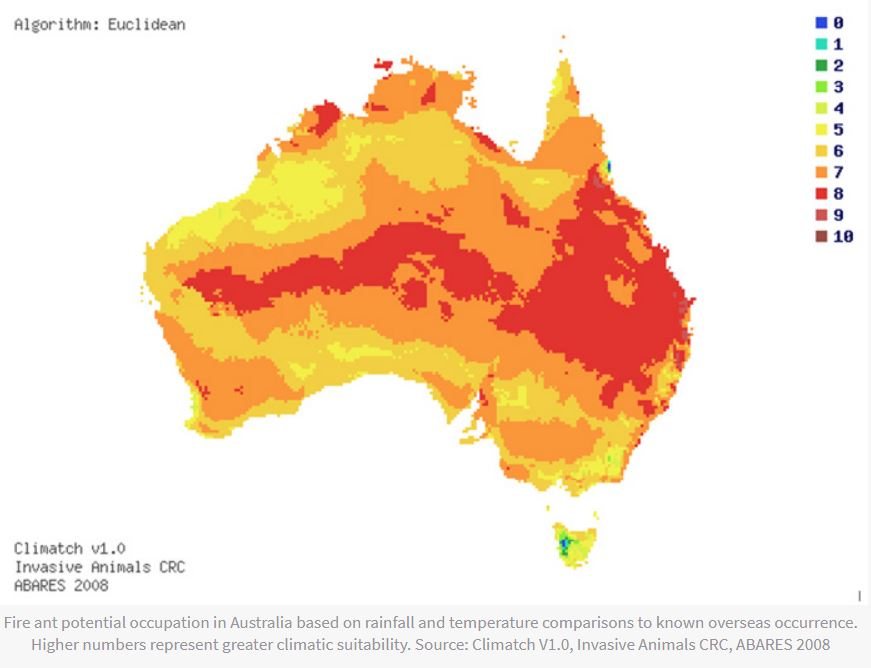
\includegraphics[scale=0.2]{map.JPG}
\caption{Potential occupation (area suitability) based on rainfall and temperature comparison with overseas invasions}
\end{minipage}
\begin{minipage}{0.4\textwidth}
\centering
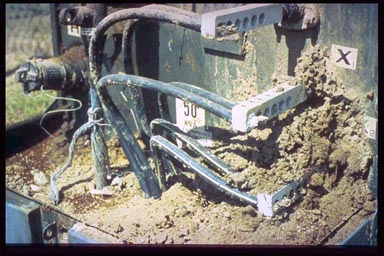
\includegraphics[scale=0.2]{RIFA_electrical.jpg}
\caption{Damage to electrical equipment}
\end{minipage}%
\begin{minipage}{0.4\textwidth}
\centering
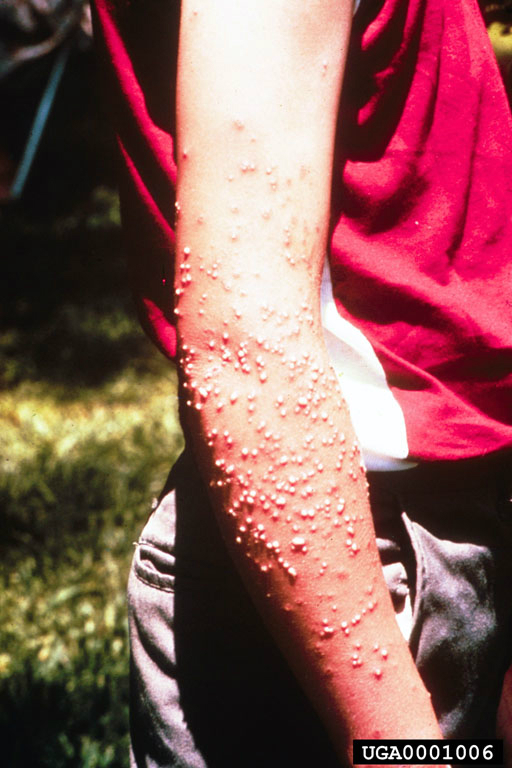
\includegraphics[scale=0.1]{rifa_stings.png}
\caption{RIFA stings}
\end{minipage}
\end{figure}
\end{frame}

\section{Why and Importance Sampling Approach}

\begin{frame}
\frametitle{Why an Importance Sampling Approach}
\begin{itemize}
\setlength\itemsep{2em}
\item In some cases, it is possible to obtain analytical solutions to compute the evolving sequence of posterior distributions, however, data is often complex and analytical solutions might be precluded.
\itemSequential Monte Carlo methods are one of many solutions that can deal with this issue. 
If we have many samples from the posterior distribution we can approximate the posterior. 
\item When it is impossible to obtain samples from these distributions directly we can use alternative Monte Carlo methods, like Importance Sampling.
\item Importance Sampling however has the drawback that every time new data becomes available, one needs to recompute the importance weights over the entire state sequence. this means that as the time increases the computational complexity increases.
Sequential importance sampling is a modification of Importance Sampling that can overcome this problem.
\end{itemize}
\end{frame}

\begin{frame}
\frametitle{Other Applications}
\begin{itemize}
\setlength\itemsep{2em}
\item We can envisage the approach being used to study the evolution of a species’ geographic range, for both invasive and non invasive species. 
\item The algorithm could be also applied to a variety of other missing data problems where new incomplete data is continuously  acquired, like  in  crime  prediction, o  bushfire modeling. 
\item Another potential application is in the study of the spread of infectious diseases, where observations are made in the form of diagnosed cases, but  missing  data  in  the  form  of  undiagnosed  cases  is unavoidable.
\end{itemize}
\end{frame}

\section{Application to an AR(1) Model}

\begin{frame}
\frametitle{Application to an AR(1) Toy Model}
\begin{itemize}
\setlength\itemsep{2em}
\item This new method has been firstly applied to an AR(1) model with missing data and exact observations.
\item This Ar(1) model will be Gaussian, linear and stationary.
\item The values of expectation and variance for the normally distributed missing values in the AR(1) model can be solved analytically. This analytical estimations will be used as gold standard to prove the validity of the new method.
\end{itemize}
\end{frame}

\section{Literature Review }
\subsection{Missing Data}

\begin{frame}
\frametitle{Literature Review (Missing Data)}
\begin{itemize}
\setlength\itemsep{2em}
\item Particle filters are used to estimate a hidden state when partial (noisy) observations are made. However, the standard particle filtering algorithm can diverge or its performance can severely degrade in the presence of missing data (Zhang (2015)).
\item On the other hand, multiple imputations do not use past observations and the state transition equations when estimating the probability of the hidden state knowing the observations. This can result in poor performance when the problem can be well modelled by a Markov structure (Zhang (2015)).
\item In the context of missing observations, Zhang (2015) has developed a Multiple Imputation Particle Filter (MIPF) to deal with these deficiencies. This method uses randomly drawn values (imputations) to provide a replacement for the missing data and then uses the particle filter to estimate non-linear state with the data.
\end{itemize}
\end{frame}

\subsection{Informative Data}

\begin{frame}
\frametitle{Literature Review (Informative Data)}
\begin{itemize}
\setlength\itemsep{2em}
\item Our method deals with situations where the data are informative, a situation where standard Sequential Monte Carlo methods can perform poorly.
\item Del Moral and Murray (1990) have proposed a Sequential Monte Carlo method for sampling the posterior distribution of state-space models under highly informative observation regimes. In their method they introduce a schedule of intermediate weighting and resampling times between observation times, which guide particles towards the final state.
\item A similar method was use by Finke et al. (2018) who developed a Particle MCMC algorithm to estimate the demographic parameters of a population then incorporate this algorithm into a Sequential Monte Carlo sampler in order to perform model comparison motivated by the fact that a simple importance sampling performs poorly if there is a strong mismatch between the prior and the posterior, which is common when the data is highly informative.
\end{itemize}
\end{frame}

\section{Method}

\begin{frame}
\frametitle{Method}
\begin{itemize}
\setlength\itemsep{1em}
\item We will have a vector $\bm x^{(t)}$ for the state space, modelled on a linear, Gaussian and stationary AR(1) model. 
\item We will have a triangular matrix of observations $\bm{Z}^{(t)}$ which will store the value of the observation at each time for each time, and that will store a dash at the time points where we don't have an observation. 
\item We will then define another triangular matrix of observations  $\bm{B}^{(t)}$ of 0s (no observations) and 1s (observations) which is defined by the matrix of observations $\bm{Z}^{(t)}$. \item When I don't have an observation I will simulate from a Bernoulli distribution.
\item We will want to determine the posterior distribution of the pair 
    \[
    p(\bm{x}^{(t)}, \bm{B}^{(t)} | \bm{Z}^{(t)}).
    \]
\end{itemize}
\end{frame}

\begin{frame}
\frametitle{Method}
\begin{itemize}
\setlength\itemsep{2em}
This posterior distribution in a partially observed space is obtained re-normalising the prior distribution $q(\bm{x}^{(t)}, \bm{B}^{(t)} | \bm{Z}^{(t-1)}) $ over values consistent with $\bm{Z}^{(t)}$
\[
p(\bm{x}^{(t)}, \bm{B}^{(t)} | \bm{Z}^{(t)})  =   
\frac{ q(\bm{x}^{(t)}, \bm{B}^{(t)}|\bm{Z}^{(t-1)})} {r(\bm{z}^{(t)} | \bm{Z}^{(t-1)})}
\]
where 
\[
r(\bm{z}^{(t)} | \bm{Z}^{(t-1)}) = \int q(\bm{x}^{(t)}, \bm{B}^{(t)}|\bm{Z}^{(t-1)}) \prod_{\{s \leq t: b_s^{(t)} = 0\}}  dx_s^{(t)}.
\]
The prior for time $t$, $q(\bm{x}^{(t)},\bm{B}^{(t)} | \bm{Z}^{(t-1)})$ represents our knowledge about the state before we observe $\bm{z}^{(t)}$. In our toy example, using the independence of the processes $\bm{x}$ and $\bm{B}$, we have
\[
q(\bm{x}^{(t)},\bm{B}^{(t)} | \bm{Z}^{(t-1)}) = q(\bm{x}^{(t-1)},\bm{B}^{(t-1)} | \bm{Z}^{(t-1)}) p(x_t | x_{t-1}) p(\bm{b}^{(t)} | \bm{b}^{(t-1)}).
\]
\end{itemize}
\end{frame}

\begin{frame}
\frametitle{Method}
We approximate the posterior iteratively using a Sequential Sampling Approach:
\begin{itemize}
\setlength\itemsep{2em}
    \item At each iteration we use a collection of weighted particles to represent $p(\bm{x}^{(t-1)}, \bm{B}^{(t-1)} | \bm{Z}^{(t-1)})$ from the previous iteration.
    \item We evolve these under the model to create a new set of weighted particles representing the prior for iteration $t$, namely $q(\bm{x}^{(t)},\bm{B}^{(t)} | \bm{Z}^{(t-1)})$.
    \item However, the new vector of observations is typically inconsistent with a particle.
    \begin{itemize}
        \item The coordinates at which $\bm{b}^{(t)}$ contains a 0 may not correspond to the coordinates at which $\bm{z}^{(t)}$ contains a `-'.
        \item The observed values in $\bm{z}^{(t)}$ differ from the corresponding coordinates of $\bm{x}^{(t)}$.
\end{itemize}
\item So we modify the particles to be consistent with the observations and adjust the weights (corrections).
\end{itemize}
\end{frame}

\begin{frame}
\frametitle{Method}
At each iteration, in order to simulate via a two-step process, we propose to introduce an auxiliary variable into importance sampling.
\begin{itemize}
\setlength\itemsep{2em}
\item The auxiliary variable will be the yet to be corrected sample
 $(\bm{x}^{(t)}, \bm{B}^{(t)})$.
\item We will use a projection map $\pi$ to relate the augmented space $\Omega_{\bm{Z^{(t)}}}$ containing the elements  $(\bm{x'}^{(t)}, \bm{B'}^{(t)}, \bm{x}^{(t)}, \bm{B}^{(t)})$ to the corrected state space $\Omega'$ containing $(\bm{x'}^{(t)}, \bm{B'}^{(t)})$.
\item Then we apply Importance Sampling to estimate the posterior distribution (or in general an expectation).
\end{itemize}
\end{frame}

\begin{frame}
\frametitle{Method}
For simplicity, let us call $(\bm{x}^{(t)}, \bm{B}^{(t)}) = \bm{y}^{(t)}$ and $(\bm{x'}^{(t)}, \bm{B'}^{(t)}) = \bm{y'}^{(t)}$.

Our strategy is to define a probability $p^*$ on $\Omega_{\bm{z}^{(t)}}$ such that the marginal distribution of $p^*$ on $\Omega'$ is $p$, that is:
\[
p(\bm{y'}^{(t)} | \bm{Z}^{(t)}) = \int p^*(\bm{y'}^{(t)}, \bm{y}^{(t)} | \bm{Z}^{(t)})\; d \bm{y}^{(t)}
\]
By the the disintegration theorem there exist a family of measures $\{\nu_{y'}\}_{y' \in \Omega'}$ on $\Omega_{\bm{z}^{(t)}}$ such that for every measurable Borel function $g : \Omega_{\bm{z}^{(t)}} \rightarrow [0,\infty]$:
\[
\int_{\Omega'}\int_{\pi^{-1}} g(\bm{y}) d\bm{y} d\bm{\bm{y'}} = \int_{\Omega_{\bm{z}^{(t)}}} g(\bm{y}', \bm{y}) d(\bm{y'},\bm{y})
\]
\end{frame}

\begin{frame}
\frametitle{Method}
\begin{align*}
E_{p}[f(\bm{y'}^{(t)})]  &= \int_{\Omega'} f(\bm{y'}^{(t)})\; p(\bm{y'}^{(t)} | \bm{Z}^{(t)}) d \bm{y'}^{(t)} \\
&= \int_{\Omega'} f(\bm{y'}^{(t)})\Bigg[\int_{\pi^{-1}} p^*(\bm{y'}^{(t)}, \bm{y}^{(t)} | \bm{Z}^{(t)}) d\bm{y}^{(t)}\Bigg] d\bm{y'}^{(t)} \\ 
&= \int_{\Omega_{\bm{Z}^{(t)}}} f(\pi(\bm{y'}^{(t)}, \bm{y}^{(t)}))\; p^*(\bm{y'}^{(t)}, \bm{y}^{(t)} | \bm{Z}^{(t)}) d(\bm{y'}^{(t)},\bm{y}^{(t)}) \\
&= E_{p^*}[f(\pi (\bm{y'}^{(t)}, \bm{y}^{(t)}))].
\end{align*}
Using importance sampling
\begin{align*}
&E_{p^*}[f(\pi (\bm{y'}^{(t)}, \bm{y}^{(t)})] = \\
& \int_{\Omega_{\bm{Z}^{(t)}}} f(\pi(\bm{y'}^{(t)},  \bm{y}^{(t)})) \; \frac{p^*(\bm{y'}^{(t)}, \bm{y}^{(t)}|\bm{Z}^{(t)})}{q(\bm{y'}^{(t)}, \bm{y}^{(t)} | \bm{Z}^{(t-1)})} q(\bm{y'}^{(t)}, \bm{y}^{(t)} | \bm{Z}^{(t-1)})\; d(\bm{y'}^{(t)}, \bm{y}^{(t)}) \\ &\approx \sum_{j=1}^n  w^{(t)_j}f(\pi (\bm{y'}^{(t)_j}, \bm{y}^{(t)_j})).
\end{align*}
\end{frame}

\begin{frame}
\frametitle{Method}
At this stage we will consider the substitutions to be deterministic, meaning that $\bm{x'}^{(t)}$ and $\bm{b'}^{(t)}$ are deterministic functions of $\bm{x}^{(t)}$ and $\bm{b}^{(t)}$. In this case $p^*$ will simply be:
\[
p^*(\bm{y'}^{(t)}, \bm{y}^{(t)} | \bm{Z}^{(t)}) = p(\bm{y'}^{(t)} | \bm{Z}^{(t)}) = \frac{ q(\bm{y'}^{(t)}|\bm{Z}^{(t-1)})} {r(\bm{Z}^{(t)} | \bm{Z}^{(t-1)})}
\]
and
\[
q(\bm{y'}^{(t)}, \bm{y}^{(t)} | \bm{Z}^{(t-1)}) = q(\bm{y}^{(t)} | \bm{Z}^{(t-1)})
\]
therefore the normalised weights $w^{(t)_j}$ will be:
\[
w^{(t)_j} = \frac{q(\bm{y'}^{(t)_j} | \bm{Z}^{(t-1)}) }{q(\bm{y}^{(t)_j} | \bm{Z}^{(t-1)})}\Bigg( \sum_{j=1}^n  \frac{q(\bm{y'}^{(t)_j} | \bm{Z}^{(t-1)}) }{q(\bm{y}^{(t)_j} | \bm{Z}^{(t-1)})}\Bigg)^{-1}
\]
where
\[
\frac{q(\bm{y'}^{(t)} | \bm{Z}^{(t-1)}) }{q(\bm{y}^{(t)} | \bm{Z}^{(t-1)})} = \frac{\bigg \{ \prod_{i=2}^{N}  \frac{1}{\sqrt{2 \pi \sigma^{2}}} \exp \bigg [ { - \frac{1}{2 \sigma^{2}} }  (x'_{i} - \varphi x'_{i-1})^{2} \bigg ] \bigg \} p(x'_{1}) \prod_{i=1}^{N} p^{b'_i} (1 - p)^{1-b'_{i}}  }{\bigg \{ \prod_{i=2}^{N}  \frac{1}{\sqrt{2 \pi \sigma^{2}}} \exp \bigg [ { - \frac{1}{2 \sigma^{2}} }  (x_{i} - \varphi x_{i-1})^{2} \bigg ] \bigg \} p(x_{1}) \prod_{i=1}^{N} p^{b_i} (1 - p)^{1-b_{i}} }
\]
\end{frame}

\begin{frame}
\frametitle{Method}
I am currently working on improving the method by considering non-deterministic corrections. 
In this new setting at the corrections step we will sample again all the unobserved events that had observations at adjacent times.  
We will define a probability H that will have the form
\[
H(x_s|x'_{s-1}, x'_{s+1}) = \begin{cases} p(x_s|x'_{s-1}), & \mbox{if} \quad b_s = 0  \quad \mbox{and} \quad b'_{s-1} = 1 \quad \mbox{and} \quad b'_{s+1} = 0\\ 
p(x_s|x'_{s+1}), & \mbox{if} \quad b_s = 0  \quad \mbox{and} \quad b_{s-1} = 0 \quad \mbox{and} \quad b'_{s+1} = 1\\
\frac{p(x_s|x'_{s-1})p(x'_{s+1}|x_s)}{p(x_s)}, & \mbox{if} \quad b'_s = 0  \quad \mbox{and} \quad b'_{s-1} = 1 \quad \mbox{and} \quad b'_{s+1} = 1\\
1 & \mbox{otherwise} \end{cases}
\]
This term will also have an effect on the calculation of the weights.
\end{frame}

\section{Simulations}
\begin{frame}
\frametitle{Simulations}
\begin{itemize}
\item 20 time points, 6 missing points ($p = 0.2, \varphi = 0.5, \sigma = 1$), 1,000 particles.
\item Empirical Cumulative Function vs Cumulative Distribution Function of normal non standard distribution
\end{itemize}
\begin{figure}
\begin{minipage}{0.4\textwidth}
\centering
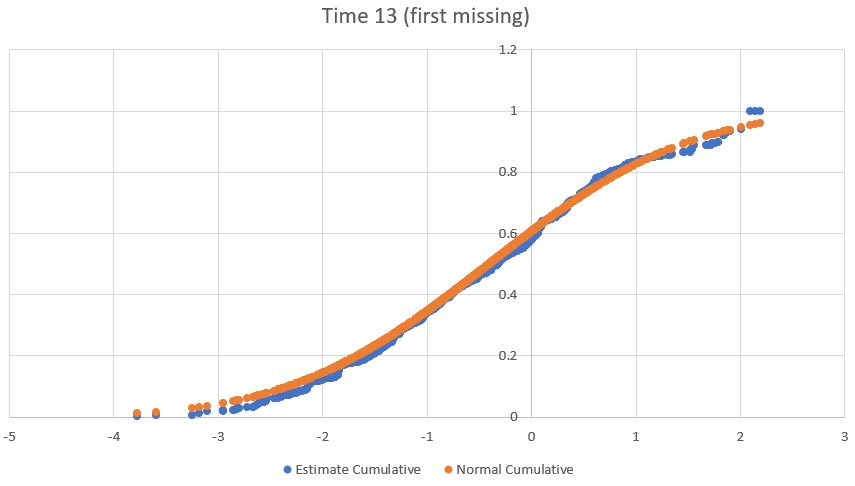
\includegraphics[scale=0.2]{im1.JPG}
\caption{ECF and CDF}
\end{minipage}
\begin{minipage}{0.4\textwidth}
\centering
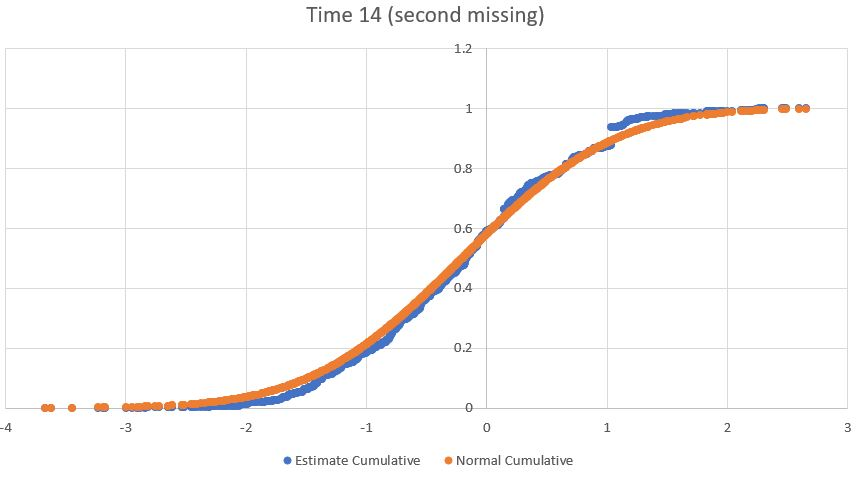
\includegraphics[scale=0.2]{im2.JPG}
\caption{ECF and CDF}
\end{minipage}%
\begin{minipage}{0.4\textwidth}
\centering
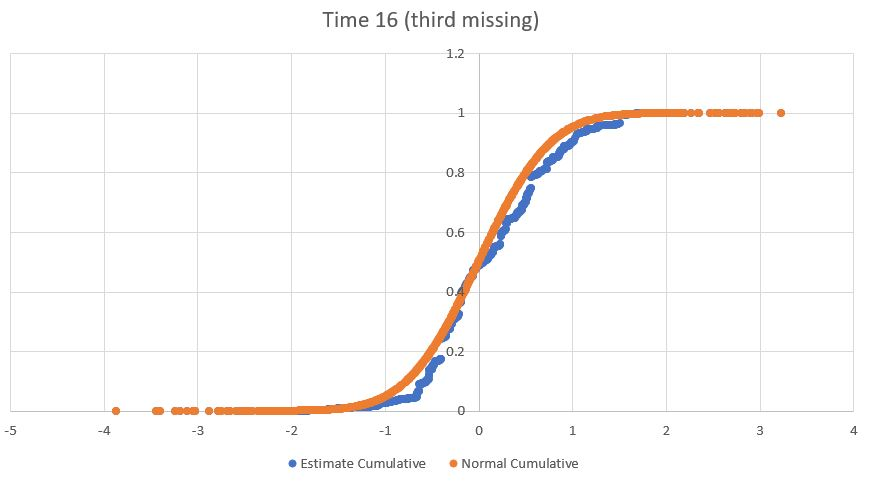
\includegraphics[scale=0.2]{im3.JPG}
\caption{ECF and CDF}
\end{minipage}
\end{figure}
\end{frame}

\section{The Analytical Solution}
\begin{frame}
\frametitle{The Analytical Solution}
\begin{itemize}
\item Could have applied a Kalman smoother or a forward-backward recursion, but I didn't find a way to do so with exact solutions.
\item But, I can also just using the definition of the AR(1) model (stationary and Gaussian)

\begin{align*}
    p(x_t | x_{\tau-1}, x_{m}) &= \mathcal{N} \Bigg(\frac{\varphi^{m-t} \sum_{i=0}^{t-\tau} \varphi^{2i} x_{m} + \varphi^{t-\tau+1} \sum_{i=0}^{m-t-1} \varphi^{2i} x_{\tau-1}}{\sum_{i=0}^{m-\tau} \varphi^{2i}}, \\
    & \frac{\sigma^2_\eta \sum_{i=0}^{m-t-1} \varphi^{2i} \sum_{i=0}^{t-\tau} \varphi^{2i}}{\sum_{i=0}^{m-\tau} \varphi^{2i}} \Bigg).
\end{align*}
Where $\tau-1$ is the index of the last observation before the block of missing values and $m$ is the fist observation after the block of missing values and $t = \tau, \dots, m-1$.

\end{itemize}
\end{frame}

\section{RIFA Model}

\begin{frame}
\frametitle{RIFA Model}
\begin{itemize}
\item New model for the RIFA invasion based on a self-exciting point process.
\item The aim is to create a model that could be faster to run than the existing model that Keith and Spring have developed.
\item This new model has the following features:
\begin{itemize}
\item It will not need to take in consideration the phylogeny of the nests (faster)
\item It considers the detection process in parallel with the founding events
\item It includes unobserved nests alongside observed nests in the detection likelihood
\end{itemize}
\item I have considered a self-exciting spatial-temporal point process for which we have a conditional intensity:
\[
\lambda(x, y, t) = \mu(x, y, t) + \int_{0}^{t} \iint_{S} g(x - x', y - y', f - f') dN(x', y', f')
\]
where $\mu$ is the background term and $g$ is the clustering density.
\item The background will be considered zero (no new nests introduced later in time) and the time and space element of the clustering density will be considered independent.
\end{itemize}
\end{frame}

\begin{frame}
\frametitle{RIFA Model}
\begin{itemize}
\item Each Parent nest will found more than one nest with $\zeta$ being the number of nests founded per nest per month and will have a maturation time $t_m$ of 8 Months.
\[
m (f - f') =
\begin{cases}
0, & \mbox{if} \quad f - f' < t_{m} \\
\zeta, & \mbox{if} \quad f - f' \geq t_{m}
\end{cases}
\]
\item The radial distance from the parent nest will be exponentially distributed, and the angular direction will be uniformly distributed 
\[
l(x - x', y - y')= J \bigg(\frac{1}{2 \pi} \sigma e^{- \sigma r}\bigg)
\]
where $J$ is the Jacobian.
\item The new nests will be killed as soon as they are detected
\[
I (t' - t) =
\begin{cases}
1, & \mbox{if} \quad t' -  t> 0 \\
0, & \mbox{otherwise}
\end{cases}
\]
Where $t'$ represents the time of detection. 
\item So the conditional intensity function will be
\[
\lambda(x, y, t) = \int_{0}^{t} \int_{0}^{t} \iint_{S} m(f - f') \cdot I(t' - t)\cdot \frac{\sigma J }{2 \pi} e^{- \sigma r} d N(x',y',t',f').
\]
\end{itemize}
\end{frame}

\begin{frame}
\frametitle{RIFA Model}
\begin{itemize}
\item The likelihood of the founding process will be that of an inhomogeneous Poisson process with density $\lambda$
\item The discovery time $t$ is known but not the founding time $f$, so the time from establishment to notification $(t - f)$ is a random variable which we consider exponentially distributed
\[
h(t_{i} - f_{i}) = \gamma \exp (- \gamma(t_{i} - f_{i}))
\]
\item The Likelihood will then be
\[
\begin{aligned}
L(s_{1}, ..., s_{n}, f_{1}, ..., f_{n}, t_{1}, ..., t_{n} | \Theta) = & \Bigg[ \prod_{j=1}^{n} \lambda(s_{j}, t_{j}) \Bigg] \times \exp \Bigg(- \int_{0}^{T} \int_{S} \lambda(s, t) d s d t \Bigg) \times \\ 
& \times \prod_{\{ i : t_{i} < T \} } h (t_{i} - f_{i}) \times \prod_{ \{ i : t_{i} = \infty \} } \int_{T}^{\infty} h(t - f_{i}) d t
\end{aligned}
\]
\item and solving

\[
\begin{aligned}
    l = & \Bigg[ \sum_{j=1}^{n} \log \lambda(s_{j},f_{j}, t_{j}) \Bigg] - \bigg(\zeta \sum_{i=1}^{n} (min\{ T, t_i \} - f_i) \bigg)  + \sum_{\{ i : t_{i} < T \} }  \bigg[\log (\gamma) -\gamma(t_{i} - f_{i}) \bigg] \\
    + & \sum_{ \{ i : t_{i} = \infty \} } \bigg[\log \bigg(\frac{1}{\gamma}\bigg) -\gamma(T - f_{i}) \bigg]
\end{aligned}
\]
\end{itemize}
\end{frame}


\section{What's Next?}

\begin{frame}
\frametitle{What's Next?}
\begin{itemize}
\setlength\itemsep{2em}
    \item Check validity of the method against the analytical solutions for the AR1 model.
    \item Find a data set with a simple model to which we can apply the method.
    \item Apply the method and the model to the data set we have for the RIFA invasion.
    \item How can we improve the code and make it faster.
    \item Will we need resampling.
\end{itemize}
\end{frame}

\section{References}

\begin{frame}[shrink=15]
\frametitle{Bibliography}
\begin{thebibliography}{}

{\small \bibitem [\protect\citeauthoryear{Beer}{1990}]{Beer} 
Beer, T.: The Australian National Bushfire model project. Math Comput. Model. 13(12), 49-56 (1990)

\bibitem [\protect\citeauthoryear{Del Moral}{2014}]{Del Moral} 
Del Moral, P., Murraly, L.M.: Sequential Monte Carlo with Highly Informative Observations. Math Comput. Model. 13(12), 49-56 (1990)

\bibitem [\protect\citeauthoryear{Keith}{2013}]{Keith} 
Keith J. M., Spring D.: Agent-based Bayesian approach to monitoring the progress of invasive species eradication programs. Pro.c Natl. Acad. Sci. 110(33): 13428-13433 (2013)

\bibitem [\protect\citeauthoryear{Malathy}{2011}]{Malathy} 
Malathy, A., Baboo, S.S.: An Enhanced Algorithm to Predict a Future Crime using Data Mining. Int. J. Comput. Appl. 21(1), 1-6 (2011)

\bibitem [\protect\citeauthoryear{Nakagawa}{2015}]{Nakagawa}
Nakagawa, S.: Missing data. In: Fox G.A., Negrete-Yankelevich S., Sosa V.J. (eds.) Ecological Statistics: Contemporary theory and application, pp 81-105. Oxford University Press (2015). 

\bibitem[\protect\citeauthoryear{O'Neill}{2002}]{O'Neill}
O'Neill, P.D., Roberts G.O.: Bayesian inference for partially observed stochastic epidemics. J. R. Stat. Soc. A. Stat. 162(1), 121-129 (2002)

\bibitem [\protect\citeauthoryear{Rubin}{1987}]{RubinMI}
Rubin, D.B.: Multiple imputation for nonresponse in surveys. Wiley, New York (1987)

\bibitem [\protect\citeauthoryear{Rubin}{1987}]{Rubin}
Rubin, D.B.: The Calculation of Posterior Distributions by Data Augmentation: Comment: A Noniterative Sampling/Importance Resampling Alternative to the Data Augmentation Algorithm for Creating a Few Imputations When Fractions of Missing Information Are Modest: The SIR Algorithm. J. Am. Stat. Assoc. 82(398), 543-546 (1987)

\bibitem [\protect\citeauthoryear{Tanner and Wong}{1987}]{Tanner}
Tanner, M.A., Wong, W.H.: The Calculation of Posterior Distributions by Data Augmentation. J. Am. Stat. Assoc. 82(398), 528-540 (1987)

\bibitem [\protect\citeauthoryear{Zhang}{2015}]{Zhang}
Zhang, X-P. et al.: Multiple Imputations Particle Filters: Convergence and Performance Analyses for Nonlinear State Estimation with Missing Data. IEEE J. Sel. Top Signa. 9(8), 1536-1547 (2015)}

\end{thebibliography}
\end{frame}






\end{document}